\documentclass{article}
\usepackage[utf8]{inputenc}
\usepackage{amsmath}
\usepackage{graphicx}
    \DeclareGraphicsExtensions{.png, .jpeg}
\usepackage{caption}
\usepackage[top=1in, bottom=1in, left=1in, right=1in]{geometry}

\title{STAT 775: Machine Learning \\ HW 04}
\author{Terence Henriod}
\date{\today}

\begin{document}

\clearpage            % All
\maketitle            % this,
\thispagestyle{empty} % removes the page number from the title page

\begin{abstract}
An exercise that shows a commonality between Ridge Regression and OLS Regression is performed and a common technique of Linear Discriminant Analysis (LDA), the Fisher Discriminant, is implemented and its performance is explored.
\end{abstract}

\newpage
\section{Exercise 01}
Elements of Statistical Learning 3.12: Show that the ridge regression estimates can be obtained by ordinary least squares regression on an augmented data set. We augment the centered matrix $\textbf{X}$ with $p$ additional rows $\sqrt{\lambda}\textbf{I}$, and augment $y$ with $p$ zeros. By introducing artificial data having response value zero, the fitting procedure is forced to shrink the coefficients toward zero. This is related to the idea of \emph{hints} due to Abu-Mostafa (1995), where model constraints are implemented by adding artificial data examples that satisfy them.

\textit{Solution}:\\
If we consider the formulae for finding the regression weight vector $\vec{\beta}$ for both methods of regression, we have for OLS Regression:
$$\hat{\vec{\beta}} = (X^{T}X)^{-1} * X^{T}\vec{y}$$
and for Ridge Regression:
$$\hat{\vec{\beta}} = (X^{T}X + \lambda\textbf{I})^{-1} * X^{T}\vec{y}^\prime$$
Let us consider the OLS Regression formula. Suppose we create an $X^\prime$ matrix and a $y^\prime$ vector as in the problem statement, where the $X$ matrix has a $p$ x $p$ matrix of $\sqrt{\lambda}\textbf{I}$ appended to the ``bottom".

Consider the $(X^{T}X)^{-1}$ term. When we compute $X^{\prime T}X^\prime$, because of the nature of matrix multiplication, the $\sqrt{\lambda}$ terms only get multiplied with one another, and only when matrix multiplication sub-operations that produce the elements of the diagonals of the result at that. This results in a result matrix equivalent to that produced by the `non-$^\prime$' version, except that $\sqrt{\lambda} * \sqrt{\lambda} = \lambda$ is added to each diagonal element. Thus $X^{\prime T}X^\prime = X^{T}X + \lambda\textbf{I}$.

Now consider the $X^{T}\vec{y}$. Because $\vec{y}^\prime$ has been padded with $0$s, none of the $\sqrt{\lambda}$ terms in $X^{\prime T}$ affect the sums that compose the elements of the resulting vector in the matrix-vector multiplication of $X^{\prime T}\vec{y}^\prime$. Thus $X^{T}\vec{y} = X^{\prime T}\vec{y}^\prime$, the same result as in both regressions.

Since all elements of the augmented OLS Regression are equivalent to the terms of the Ridge Regression, the two must be equivalent.

Alternately, we can consider the $RSS$ or objective function of the OLS Regression, specifically in the augmented case:
\begin{align*}
  RSS &= \sum_{i=1}^{N + p}{(y_{i} - \sum_{j=1}^{p}{x_{ij}\beta_{j}})^{2}}\\
      &= \sum_{i=1}^{N}{(y_{i} - \sum_{j=1}^{p}{x_{ij}\beta_{j}})^{2}} + \sum_{i=N+1}^{p}{\sum_{j=1}^{p}{(x_{ij}\beta_{j}})^{2}}\\
      &= \sum_{i=1}^{N}{(y_{i} - \sum_{j=1}^{p}{x_{ij}\beta_{j}})^{2}} + \sum_{j=1}^{p}{\lambda\beta_{j}^{2}}
\end{align*}
which is the objective function for Ridge Regression. Note that the sum inside the sum in the second term of the intermediate step will add a lot of zeros with the occasional $(\sqrt{\lambda}\beta)^{2}$.

%
\newpage
\section{Exercise 02}
\subsection{Problem Statement}
Using the zip code digit data from the ESL website, use the Fisher Discriminant to perform binary classification between 2s and 3s, 4s and 5s, and 7s and 9s.

\subsection{Results}
Two decision boundaries were used, and both produced the same results. Let $\vec{u}$ be the line the data is projected onto for optimal discrimination. For the first method, let the decision boundary value $c = \vec{u}^{t} * \frac{1}{/2} * (\mu_{1} + \mu_{2})$, where if $\vec{u}^{t} * x_{i} > c$, then $x_{i}$ belongs to the first class, or the other class otherwise. For the second, the data was projected onto $\vec{u}$, and then a gaussian distribution was fitted to the projected points for each class, and then using Bayes' Rule, a decision boundary was computed. IT must be that either the data were small enough, the projections were separate enough, or the covariances were similar enough that no difference between the methods was seen. It should be noted though, that the first method is requires the assumptions that each class is equally likely and have similar covariance to be valid.

The results are as follows:
 % \begin{figure}[h!]
 %    \centering
 %    \begin{minipage}{.5\textwidth}
 %      \centering
 %      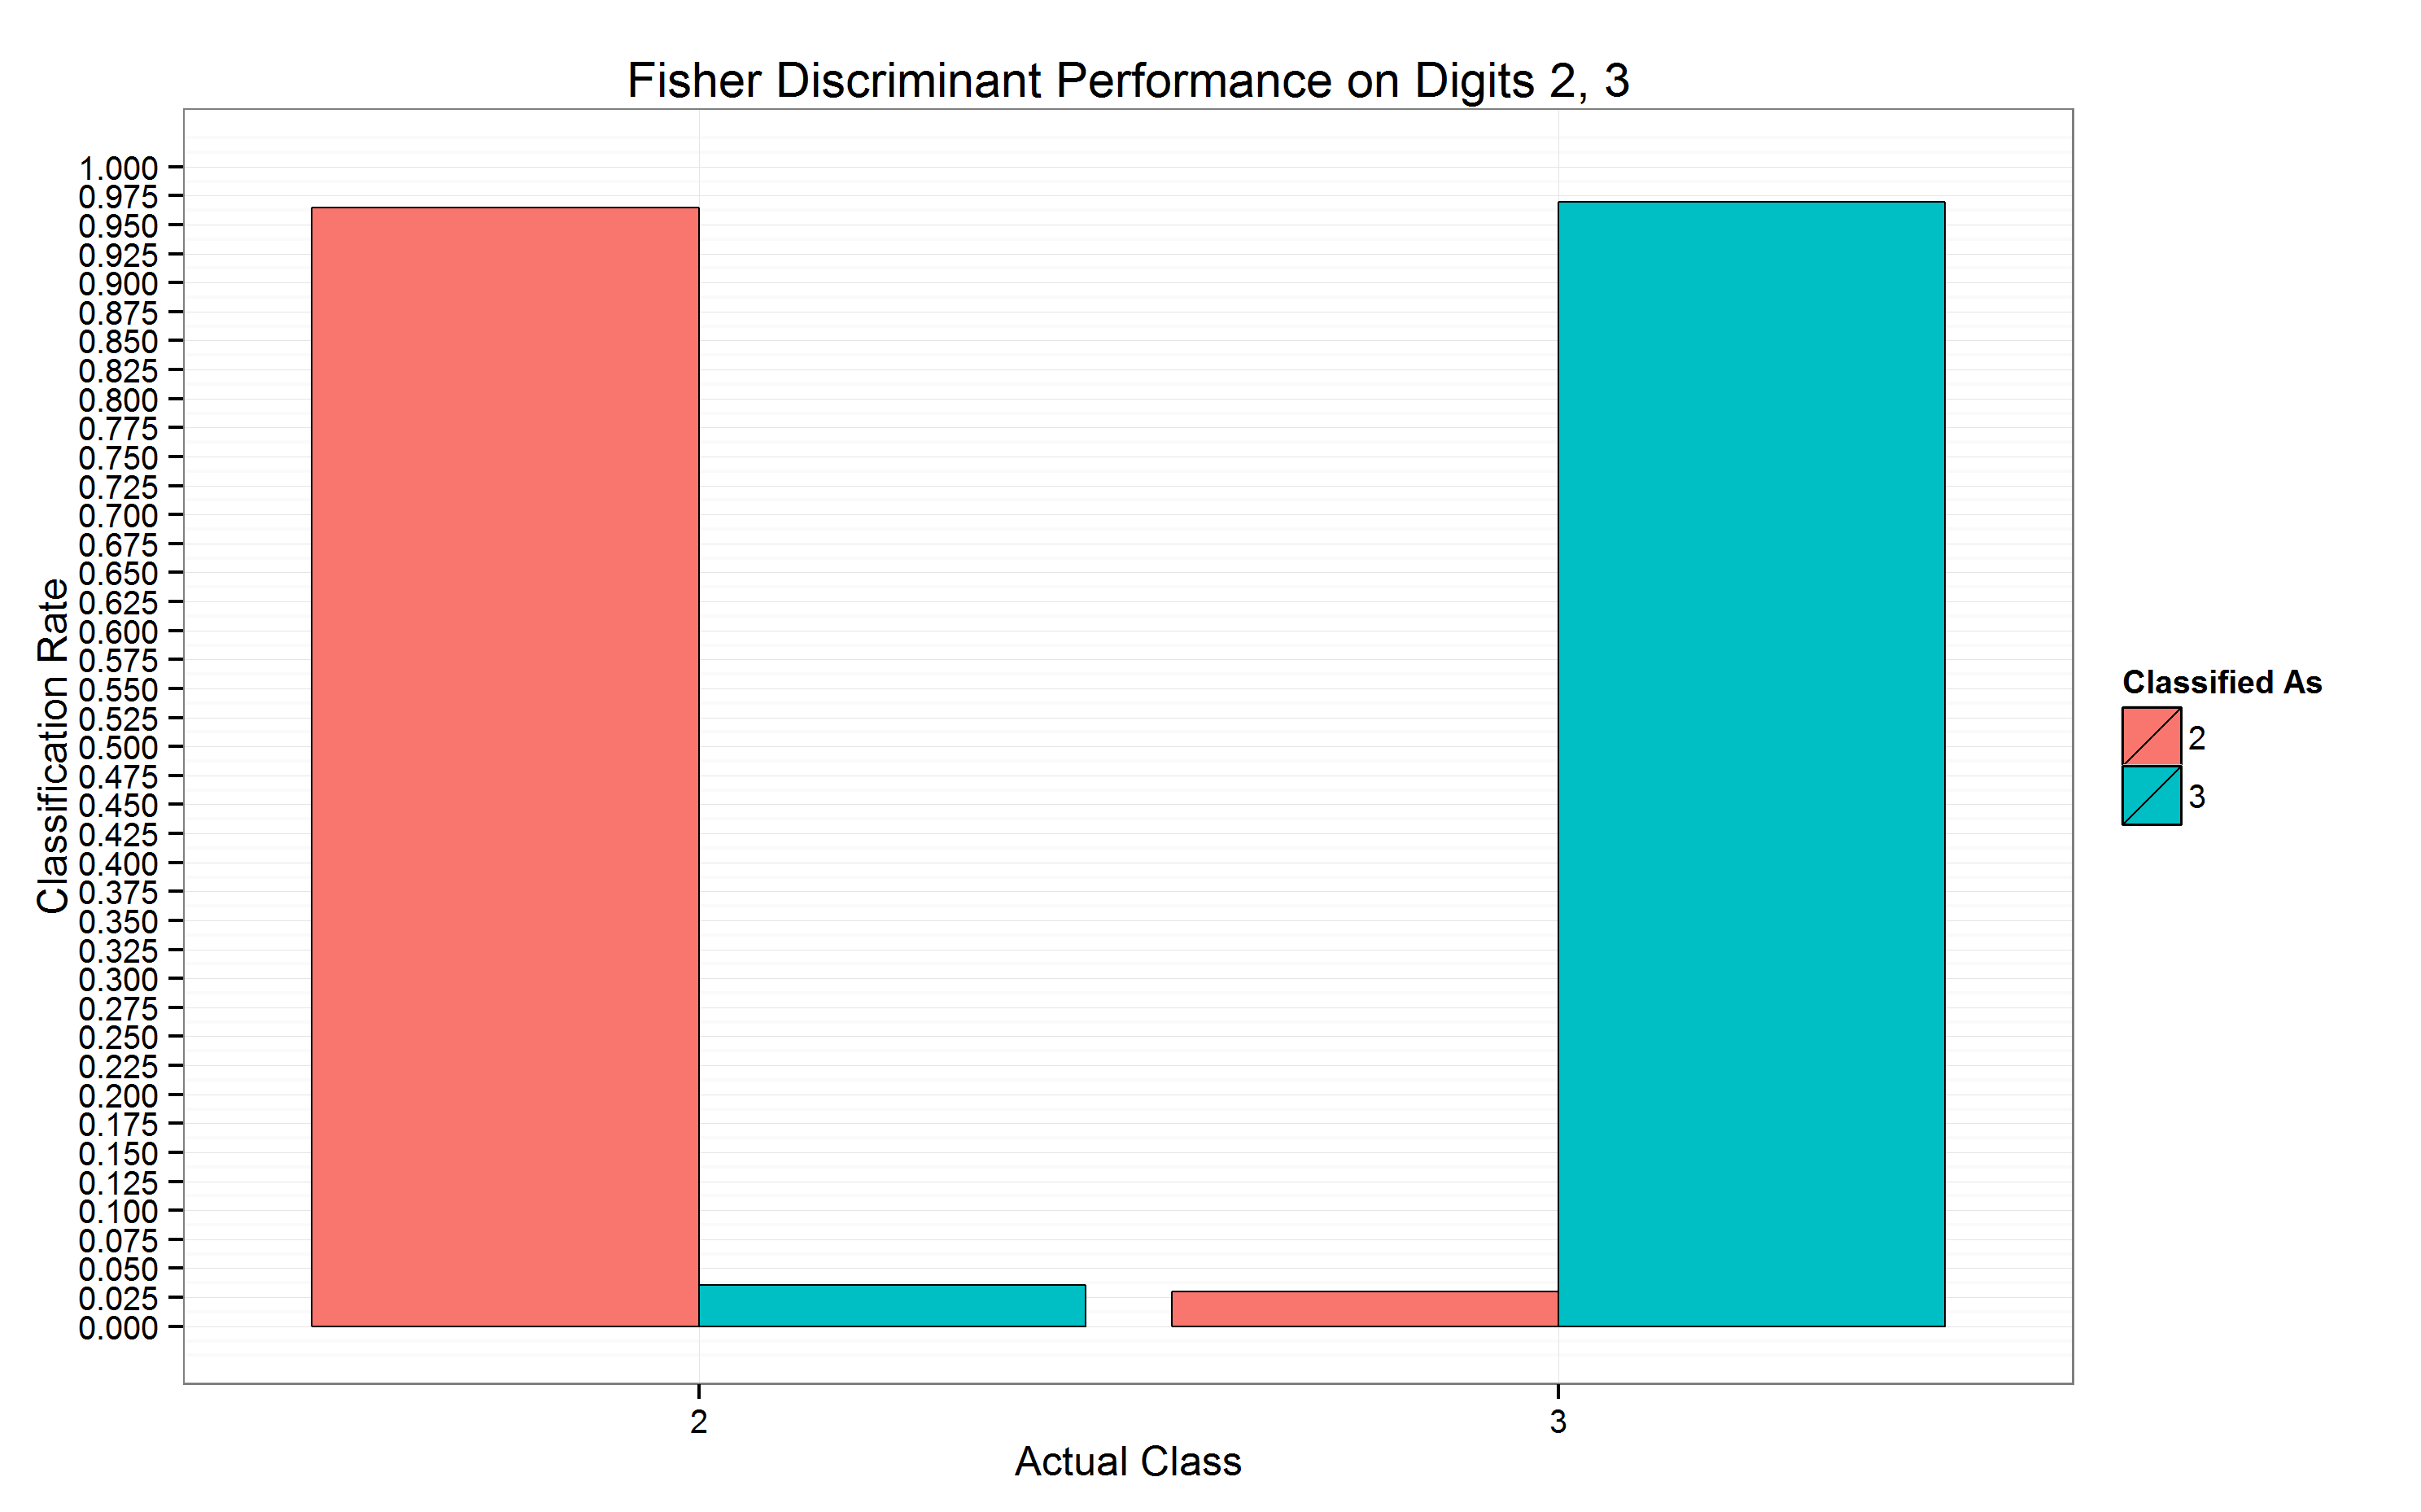
\includegraphics[width=.8\linewidth]{Fisher_Discriminant_Performance_on_Digits_2,_3}
 %      \caption{A bar chart indicating the classification/misclassification rates for 2s and 3s.}
 %      \label{fig:2_3_bar}
 %    \end{minipage}%
 %    \begin{minipage}{.5\textwidth}
 %      \centering
 %      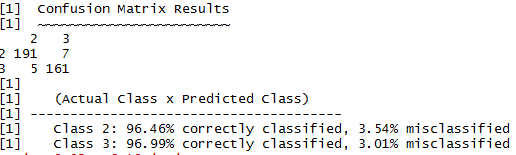
\includegraphics[width=.7\linewidth]{2_3_confusion}
 %      \caption{A custom confusion-matrix-output from R indicating the classification performance of the Fisher Discriminant on 2s and 3s.}
 %      \label{fig:2_3_confusion}
 %    \end{minipage}
 %  \end{figure}

 % \begin{figure}[h!]
 %    \centering
 %    \begin{minipage}{.5\textwidth}
 %      \centering
 %      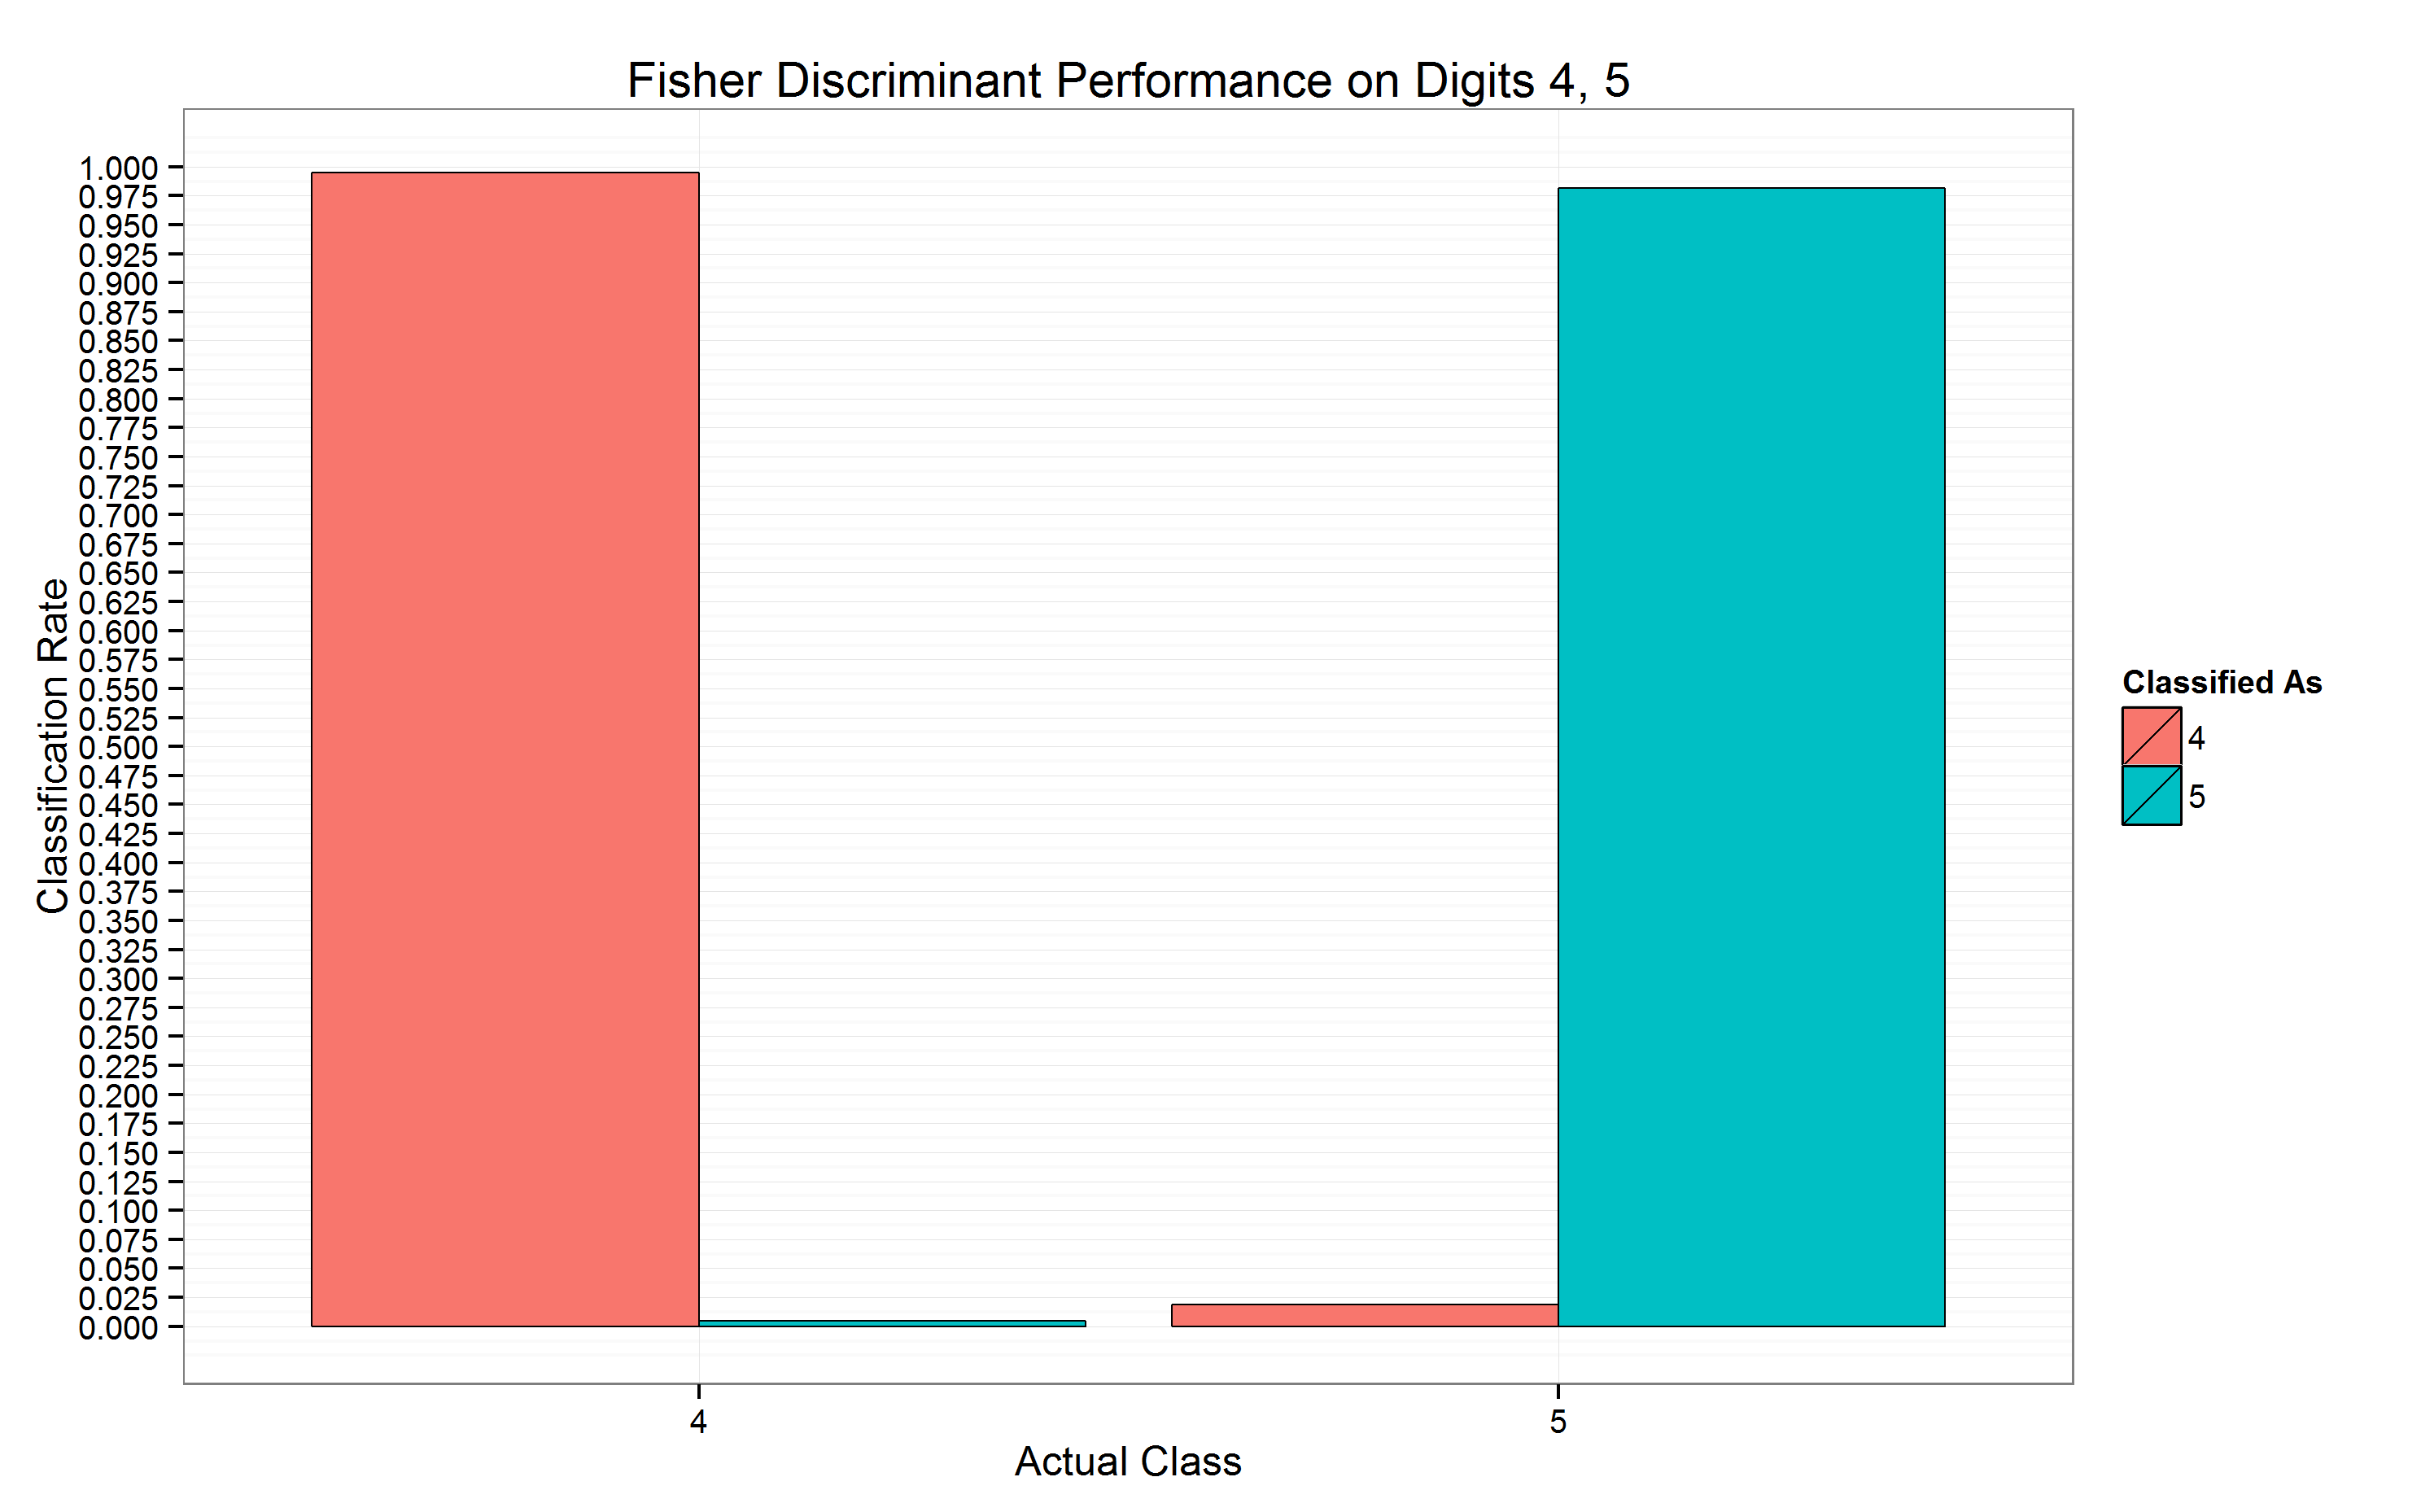
\includegraphics[width=.8\linewidth]{Fisher_Discriminant_Performance_on_Digits_4,_5}
 %      \caption{A bar chart indicating the classification/misclassification rates for 4s and 5s.}
 %      \label{fig:4_5_bar}
 %    \end{minipage}%
 %    \begin{minipage}{.5\textwidth}
 %      \centering
 %      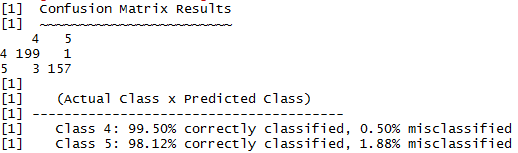
\includegraphics[width=.7\linewidth]{4_5_confusion}
 %      \caption{A custom confusion-matrix-output from R indicating the classification performance of the Fisher Discriminant on 4s and 5s.}
 %      \label{fig:4_5_confusion}
 %    \end{minipage}
 %  \end{figure}

 %   \begin{figure}[h!]
 %    \centering
 %    \begin{minipage}{.5\textwidth}
 %      \centering
 %      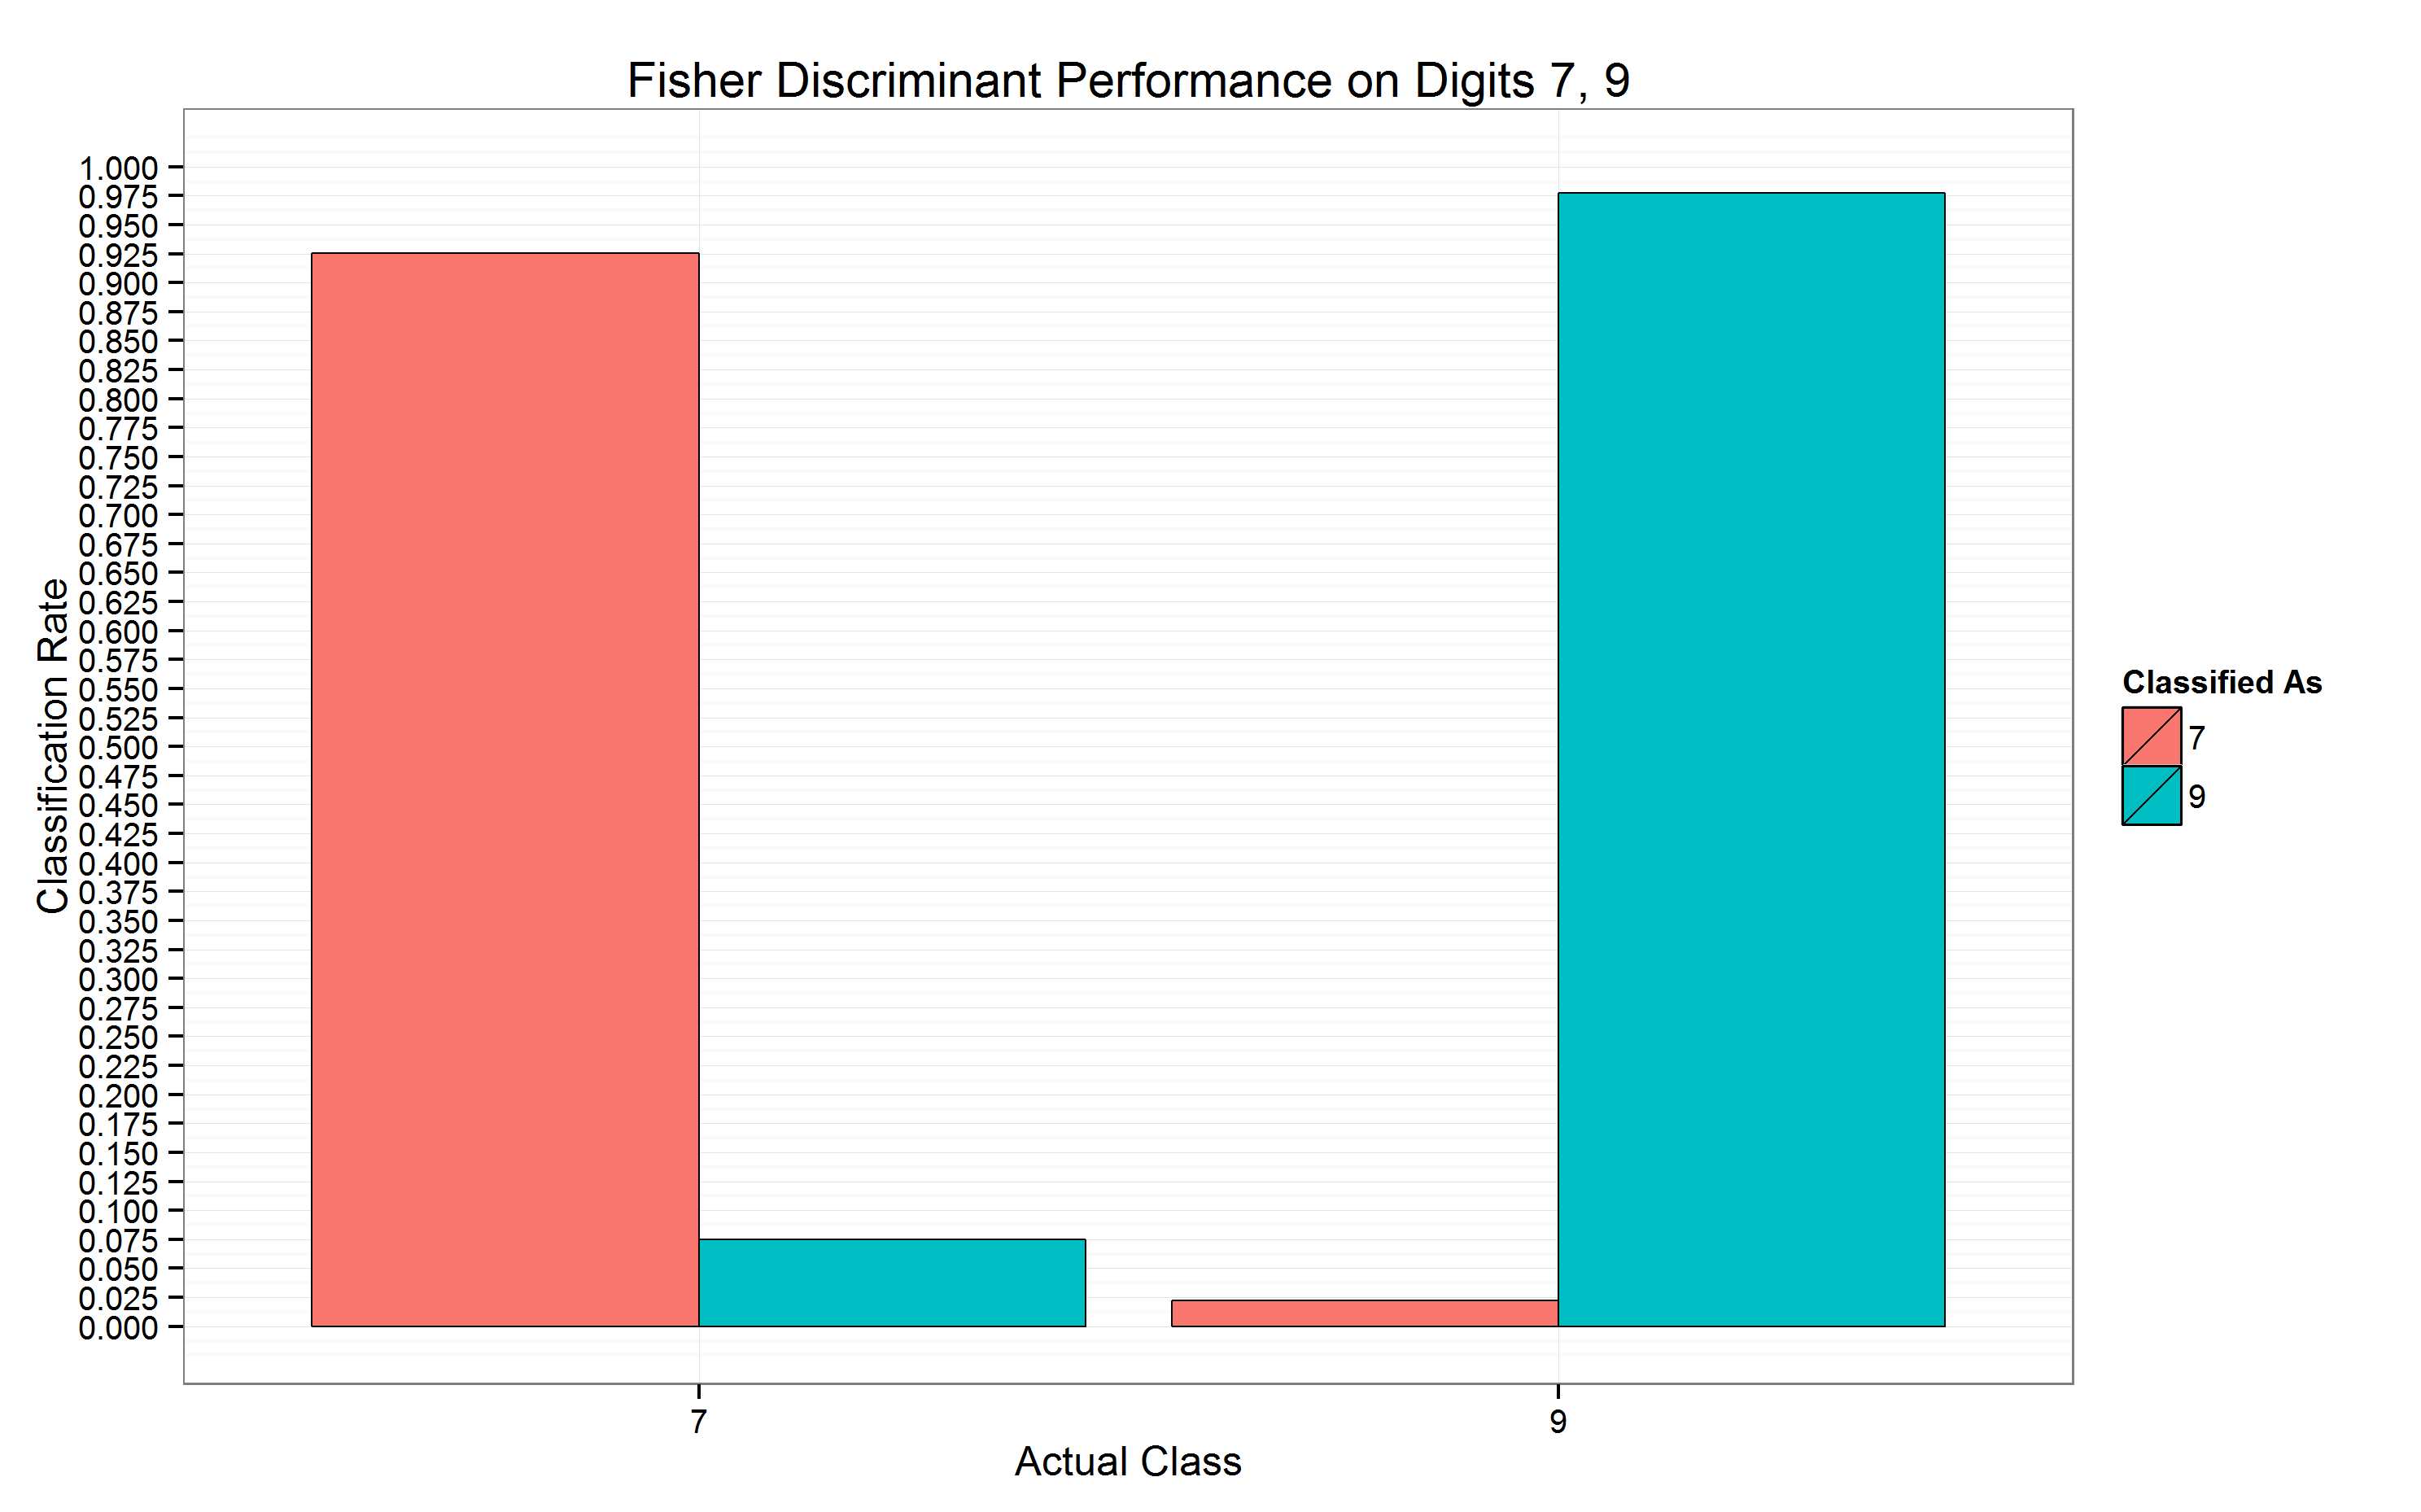
\includegraphics[width=.8\linewidth]{Fisher_Discriminant_Performance_on_Digits_7,_9}
 %      \caption{A bar chart indicating the classification/misclassification rates for 7s and 9s.}
 %      \label{fig:7_9_bar}
 %    \end{minipage}%
 %    \begin{minipage}{.5\textwidth}
 %      \centering
 %      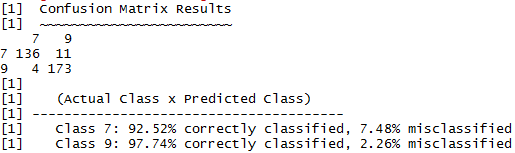
\includegraphics[width=.7\linewidth]{7_9_confusion}
 %      \caption{A custom confusion-matrix-output from R indicating the classification performance of the Fisher Discriminant on 7s and 9s.}
 %      \label{fig:7_9_confusion}
 %    \end{minipage}
 %  \end{figure}
\newpage
\begin{figure}[h!]
  \centering
  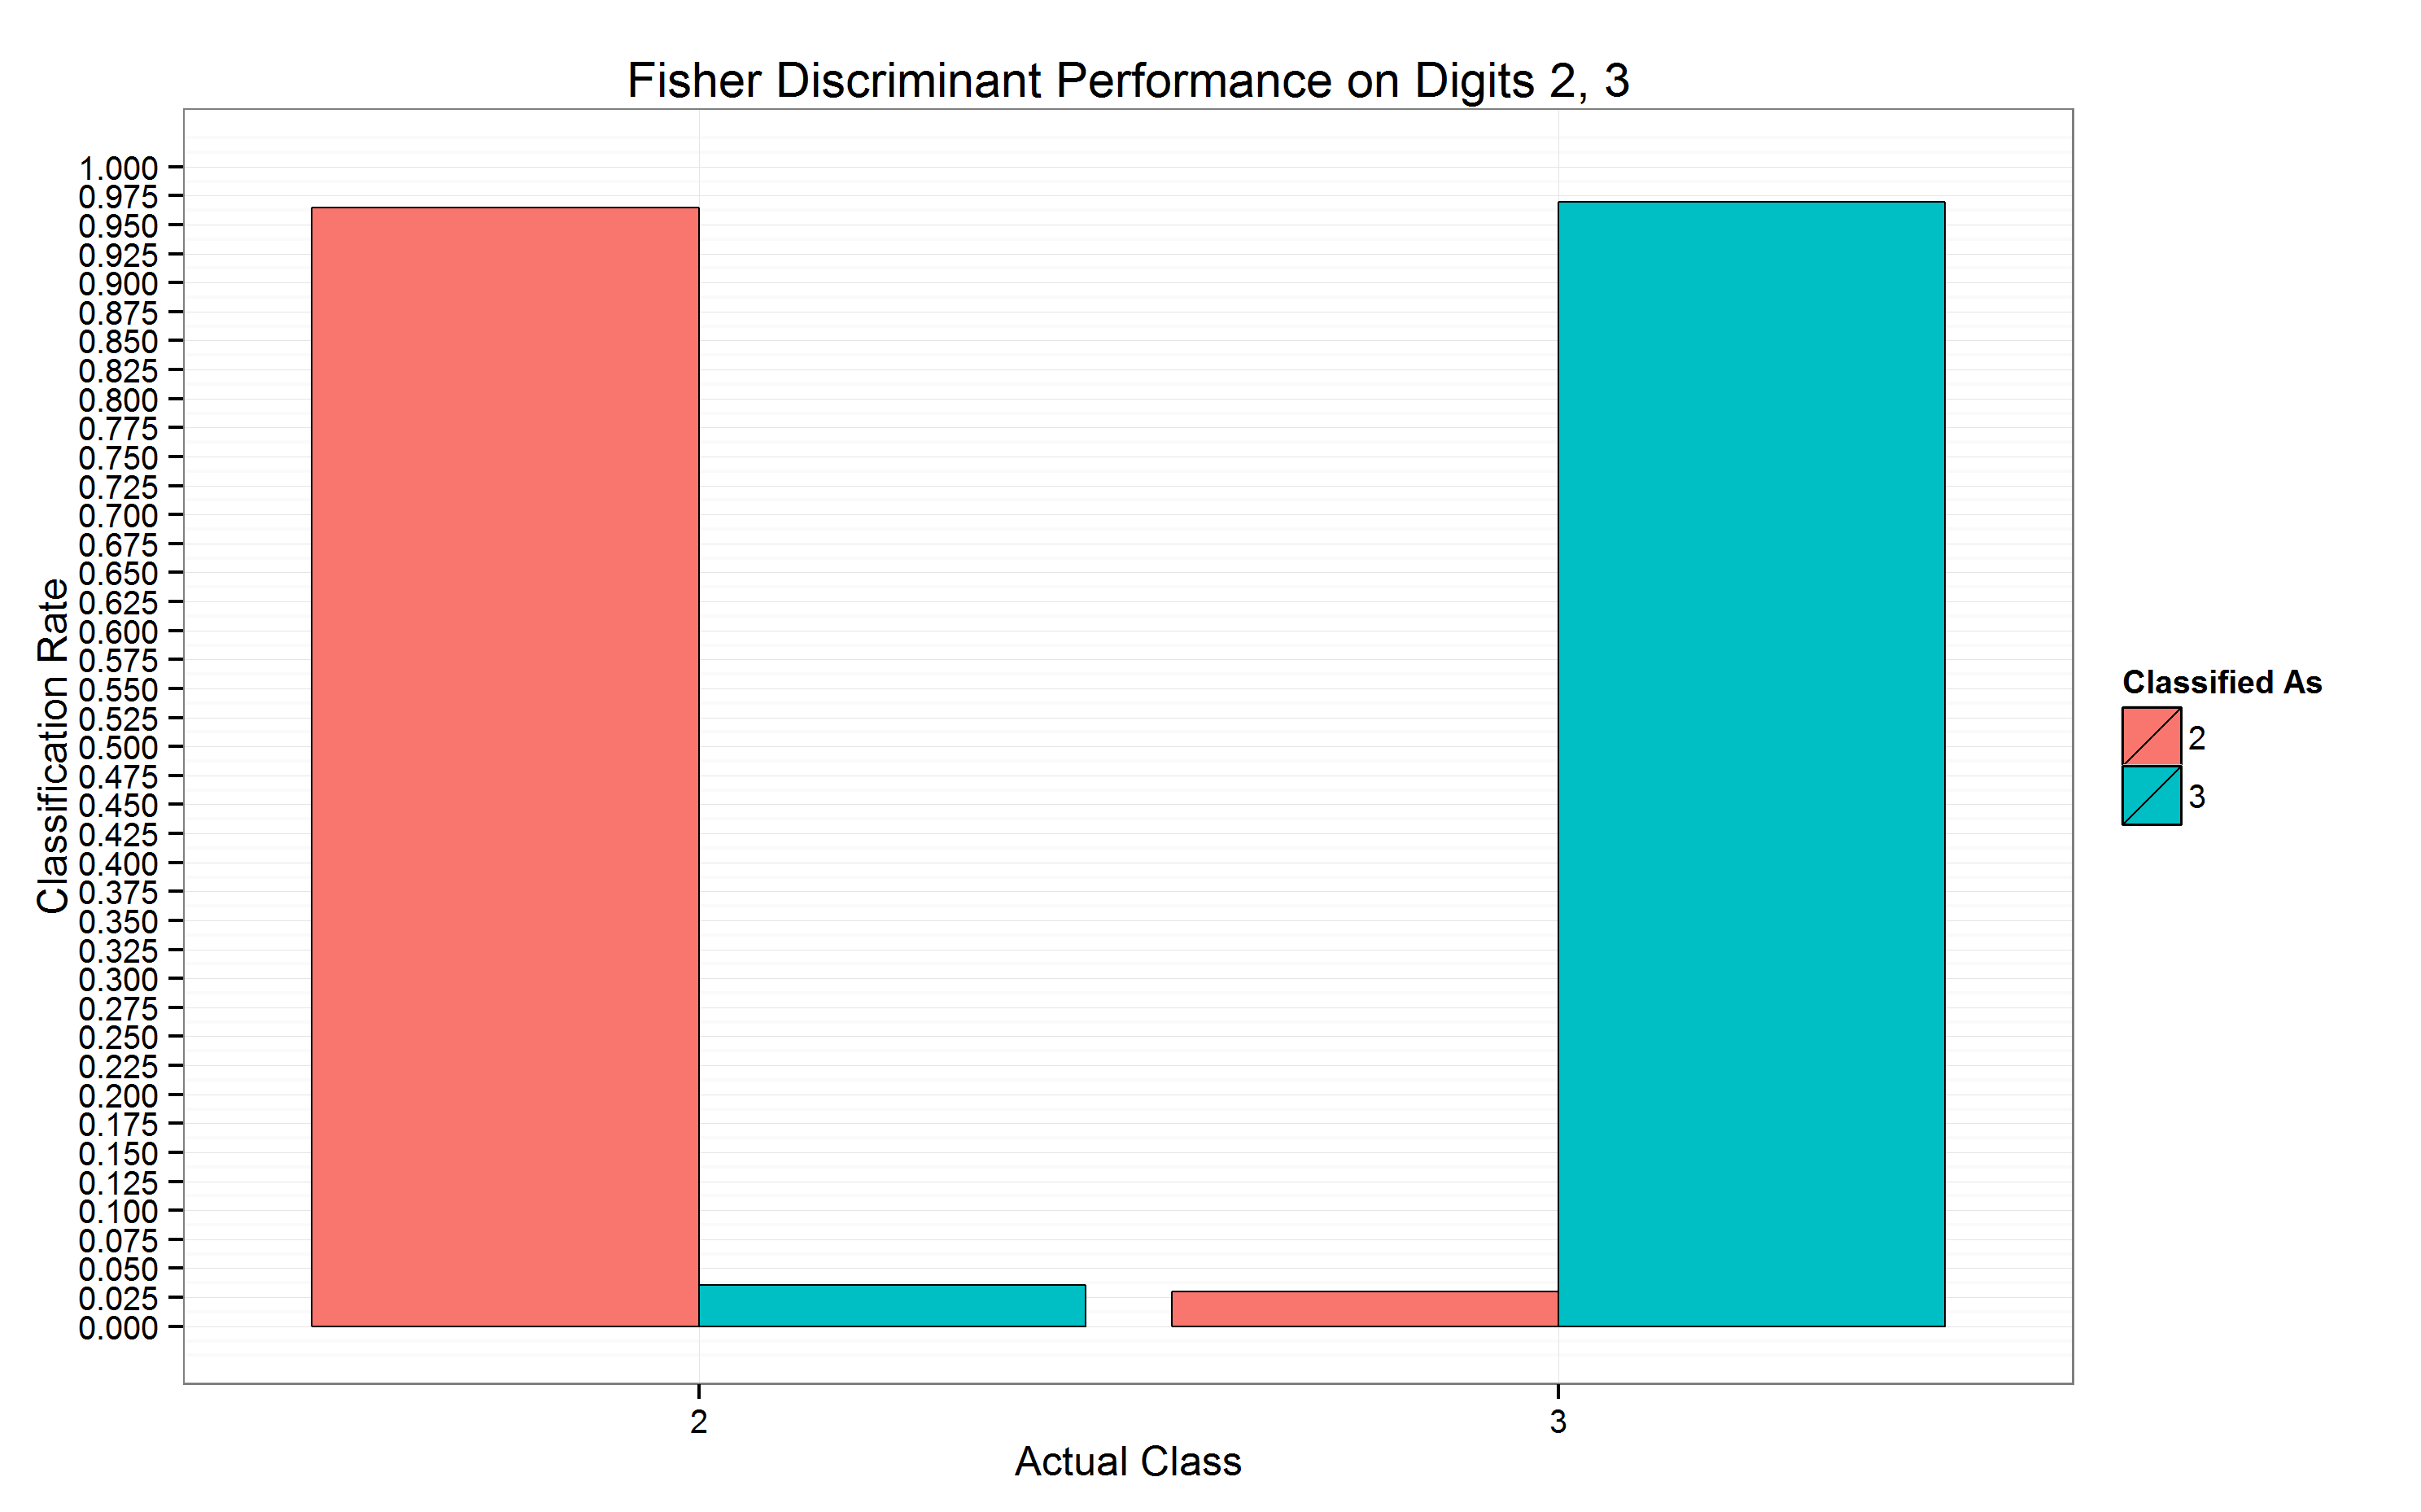
\includegraphics[width=.8\linewidth]{Fisher_Discriminant_Performance_on_Digits_2,_3}
  \caption{Classification results for Fisher Discriminant Analysis on 2s vs 3s.}
  \label{fig:2_3_bar}
\end{figure}
\begin{figure}[h!]
  \centering
  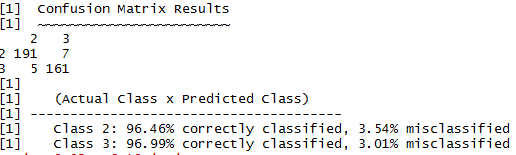
\includegraphics[width=.8\linewidth]{2_3_confusion}
  \caption{A custom confusion-matrix-output from R indicating the classification performance of the Fisher Discriminant on 2s and 3s.}
  \label{fig:2_3_confusion}
\end{figure}
%
\newpage
\begin{figure}[h!]
  \centering
  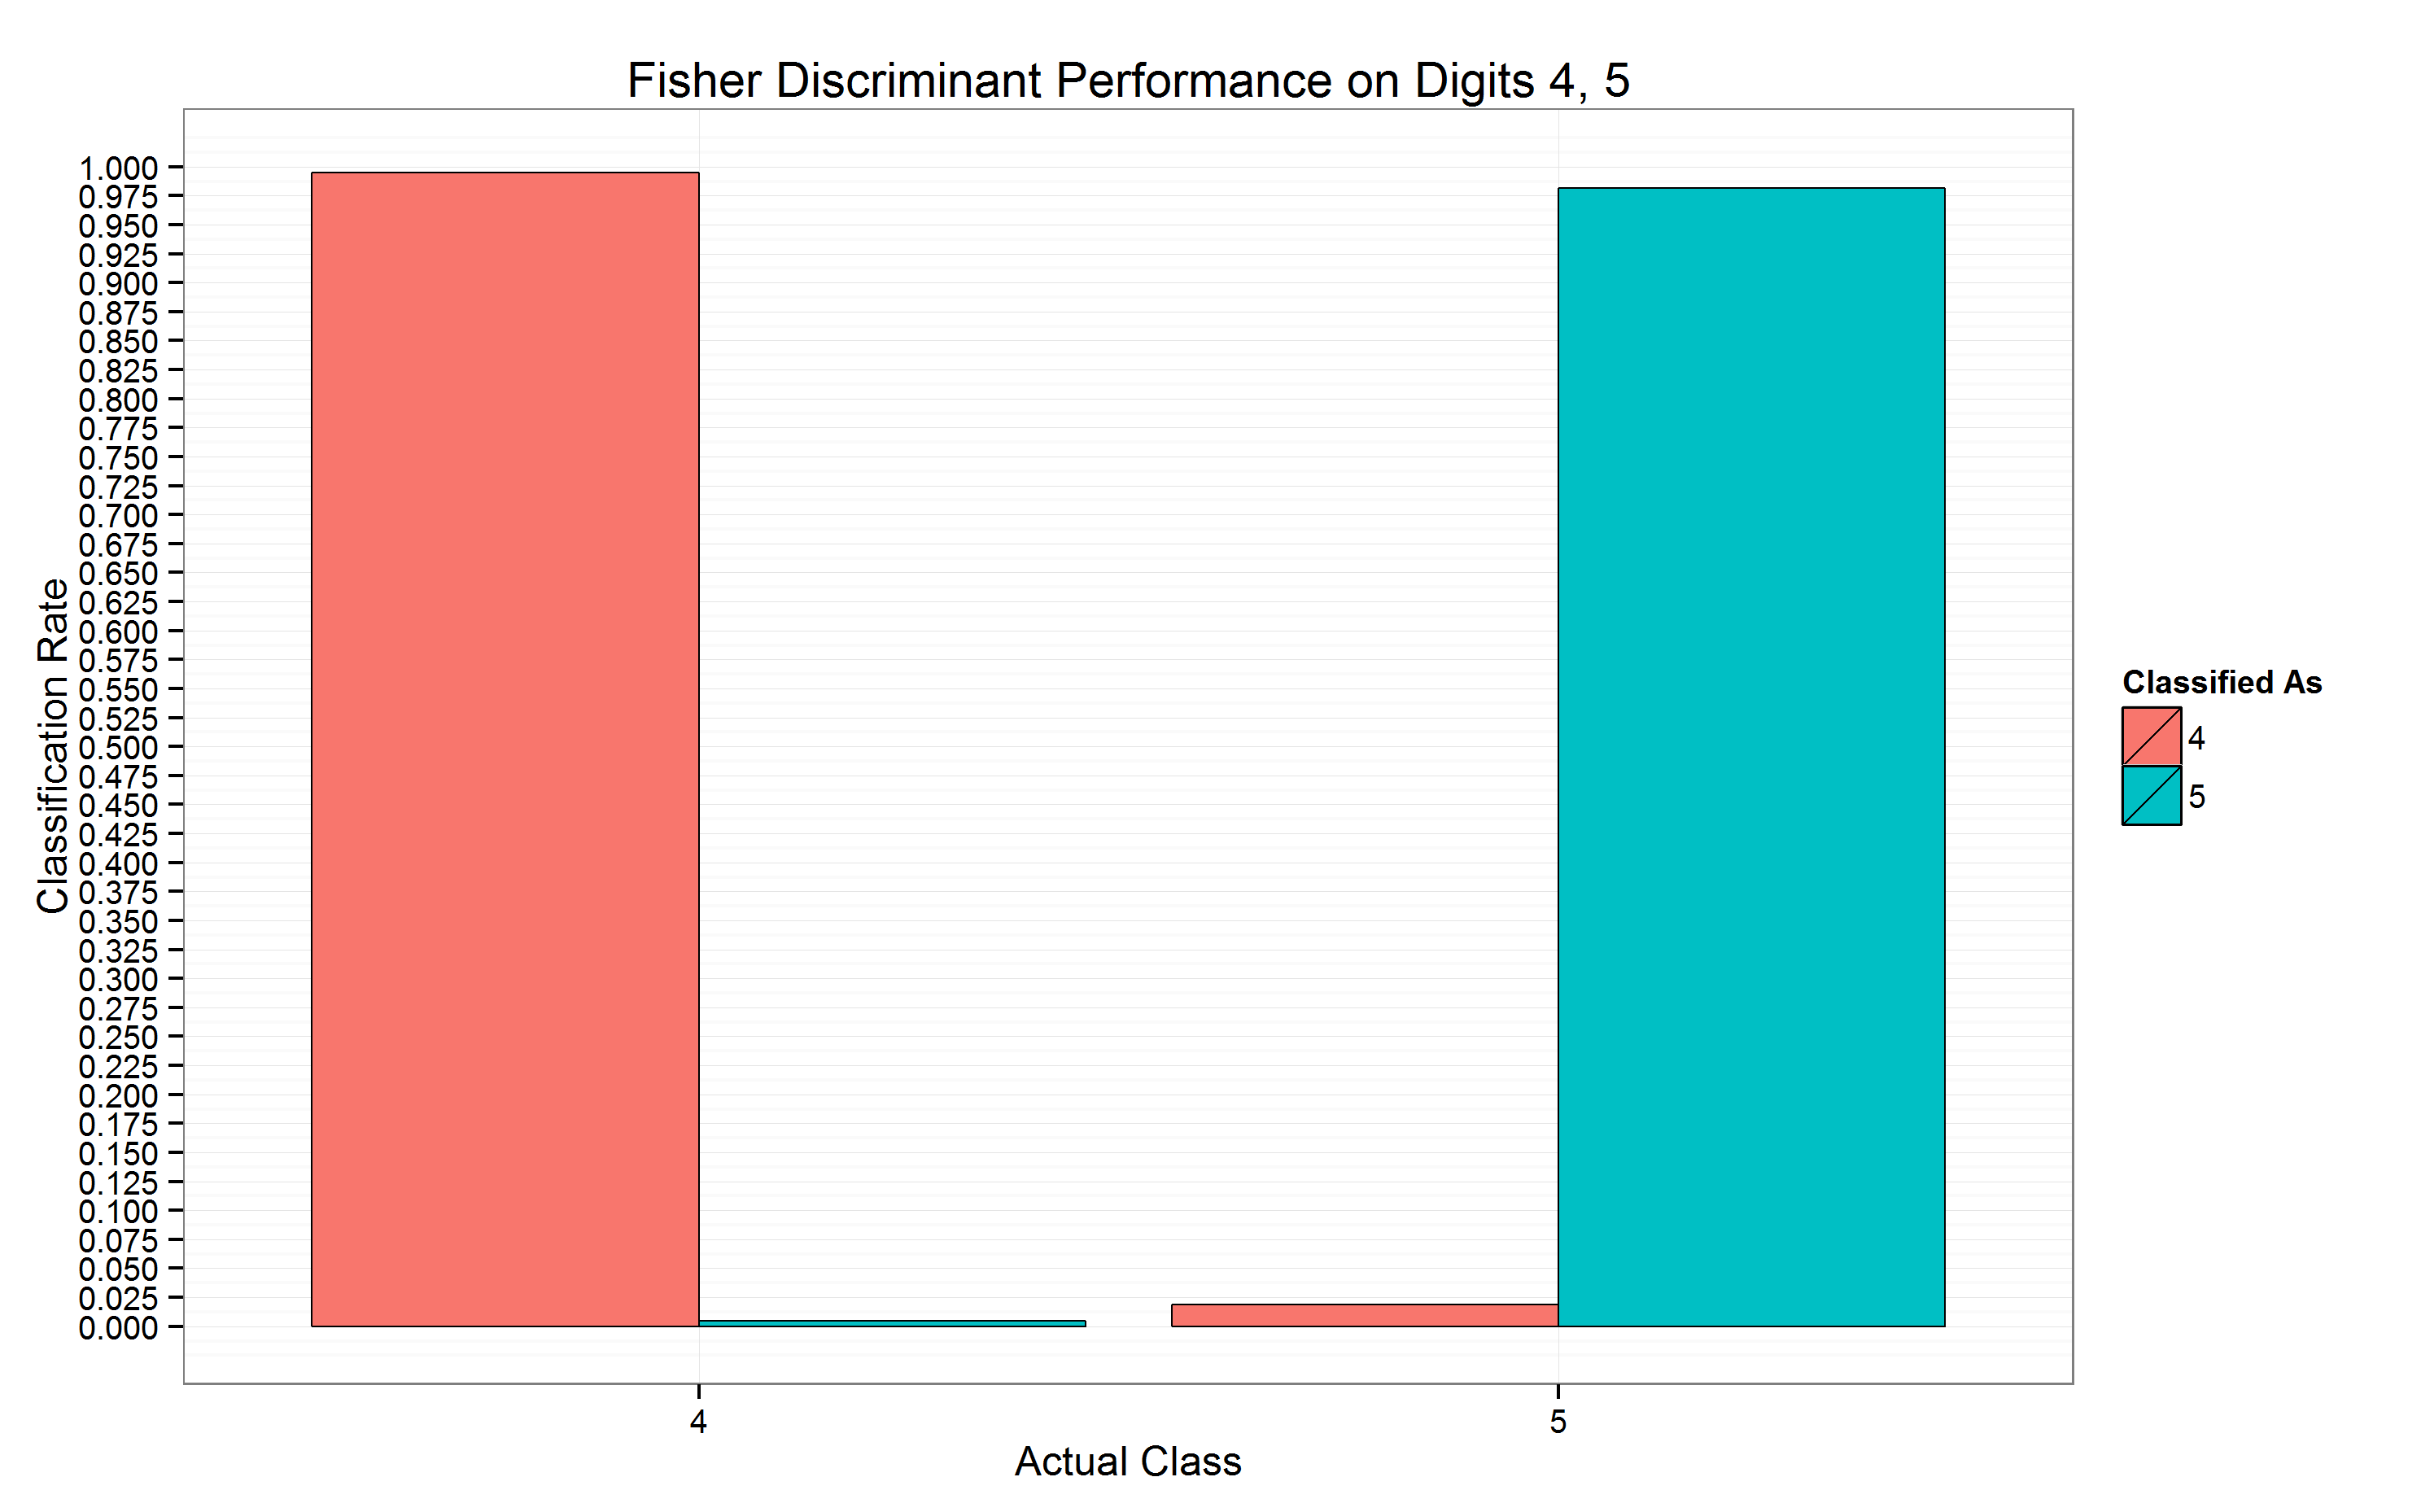
\includegraphics[width=.8\linewidth]{Fisher_Discriminant_Performance_on_Digits_4,_5}
  \caption{Classification results for Fisher Discriminant Analysis on 4s vs 5s.}
  \label{fig:4_5_bar}
\end{figure}
\begin{figure}[h!]
  \centering
  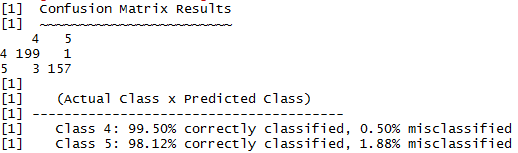
\includegraphics[width=.8\linewidth]{4_5_confusion}
  \caption{A custom confusion-matrix-output from R indicating the classification performance of the Fisher Discriminant on 4s and 5s.}
  \label{fig:4_5_confusion}
\end{figure}
%
\newpage
\begin{figure}[h!]
  \centering
  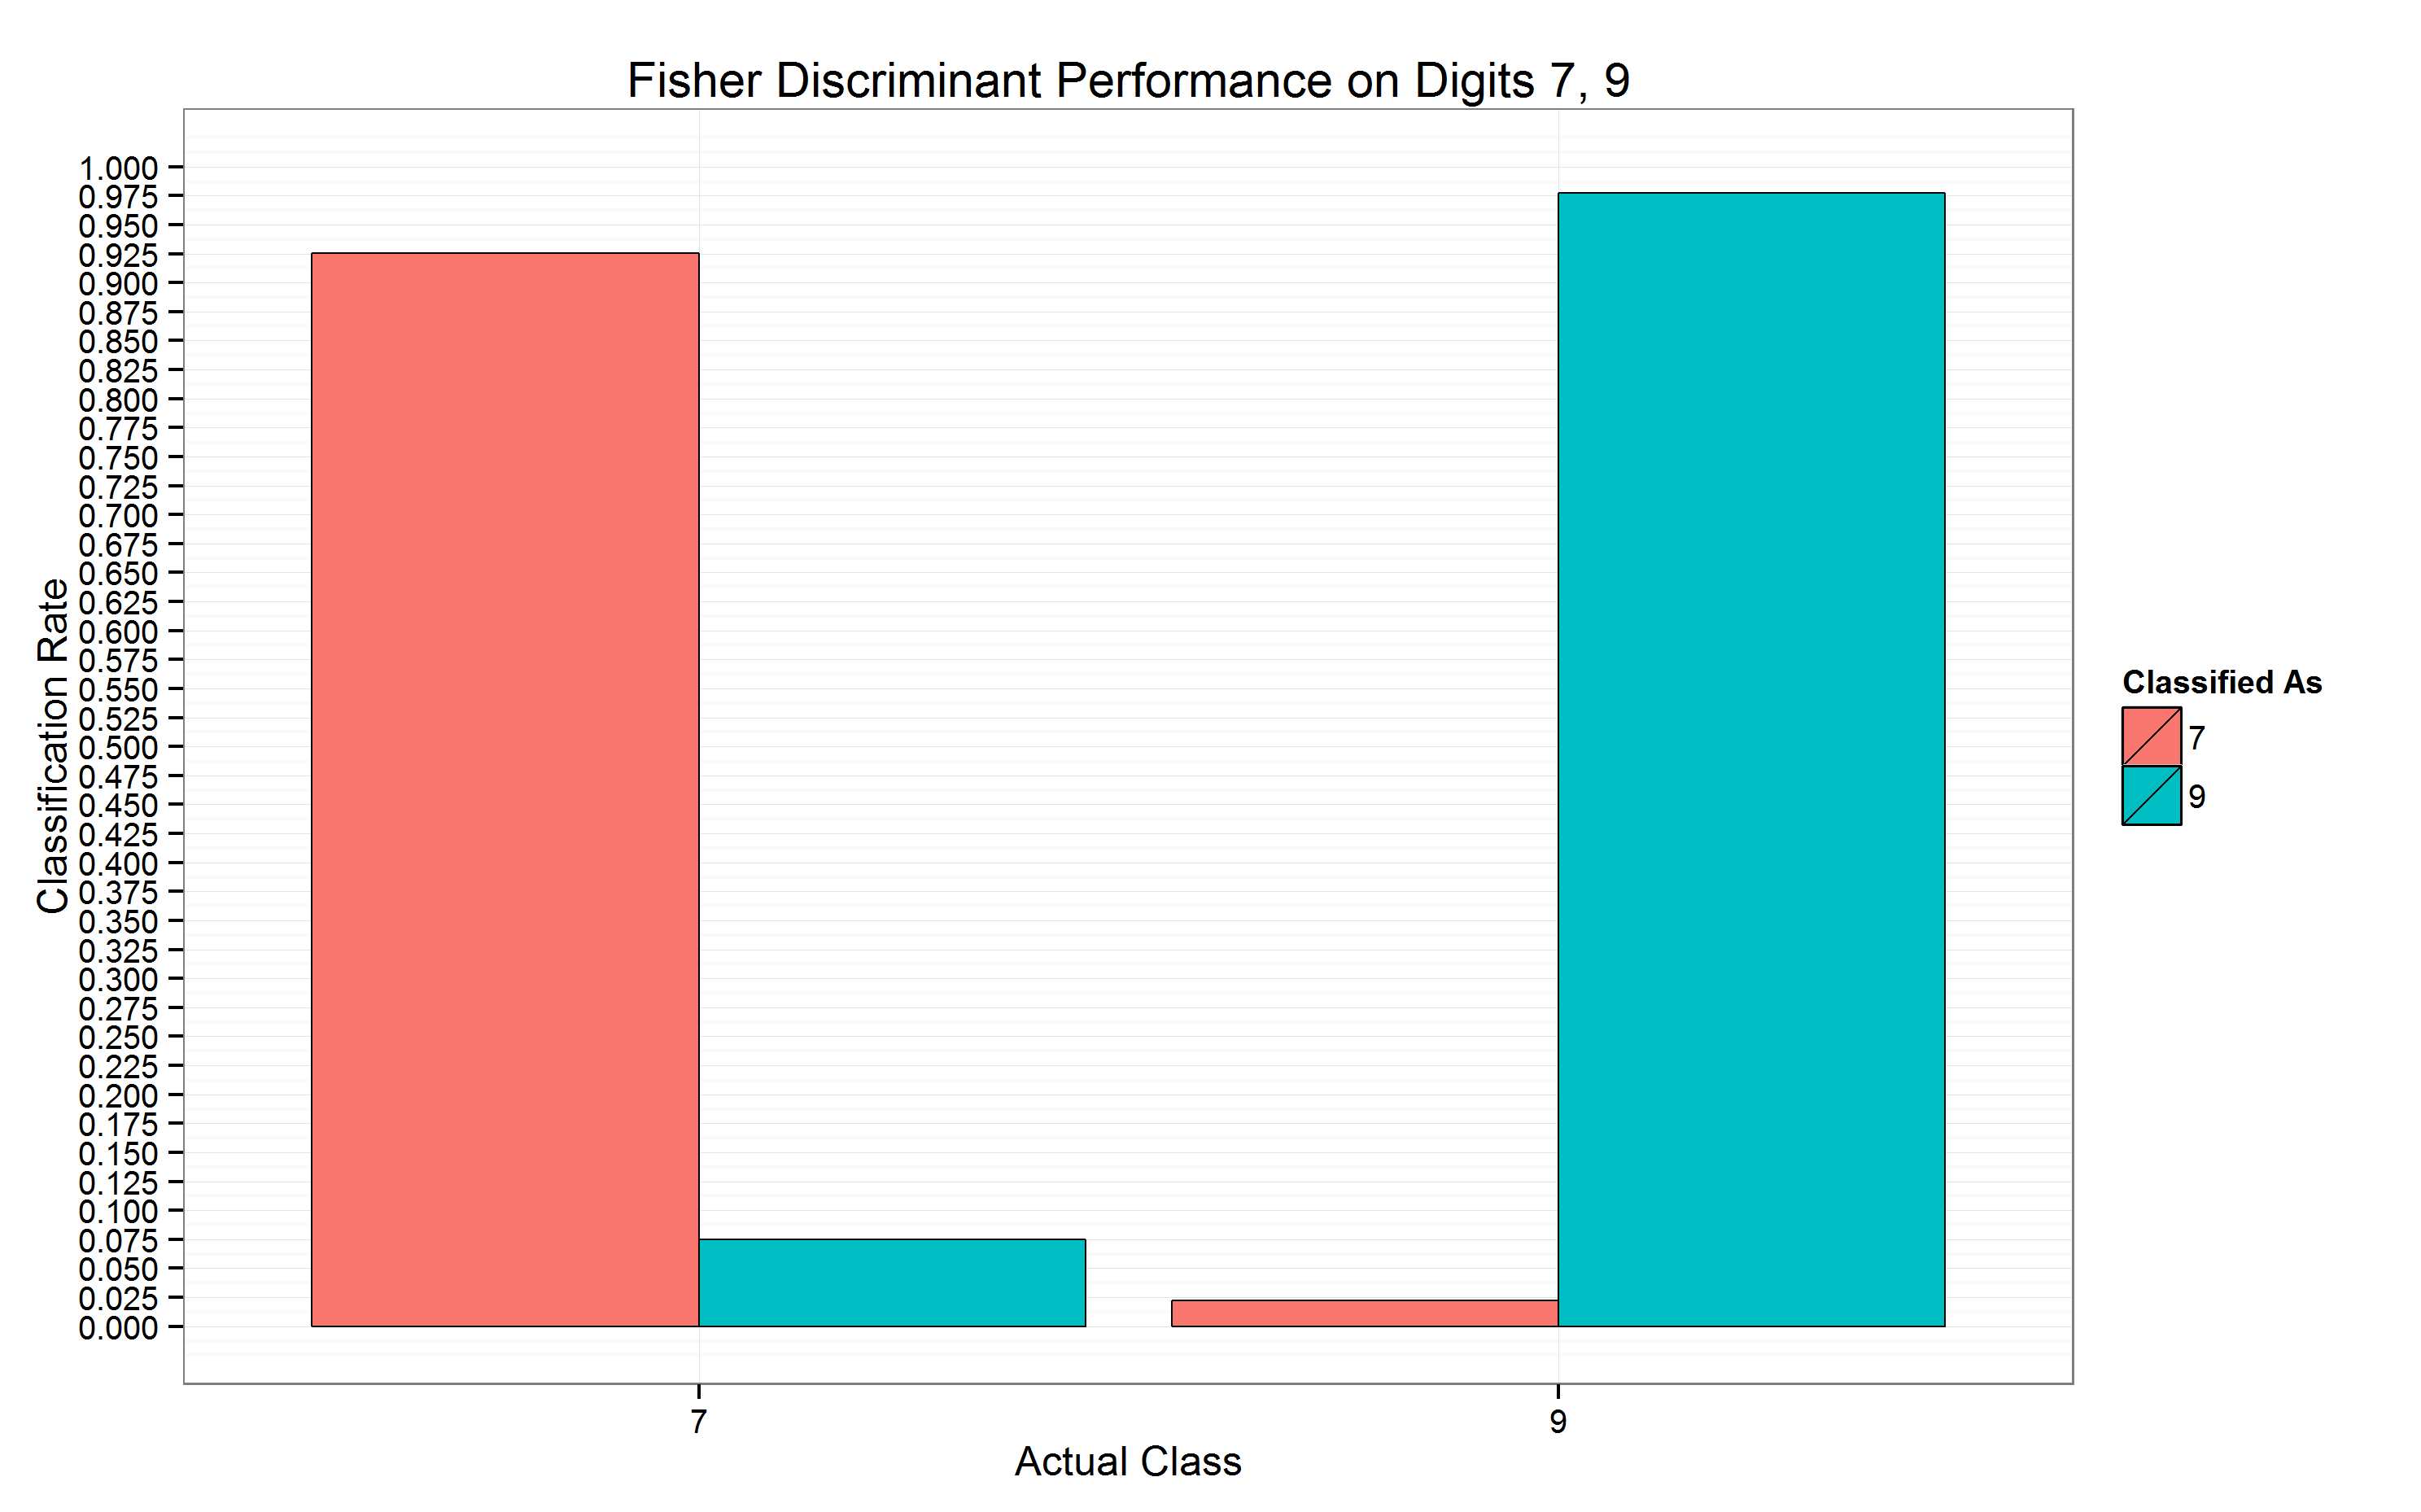
\includegraphics[width=.8\linewidth]{Fisher_Discriminant_Performance_on_Digits_7,_9}
  \caption{Classification results for Fisher Discriminant Analysis on 7s vs 9s.}
  \label{fig:7_9_bar}
\end{figure}
\begin{figure}[h!]
  \centering
  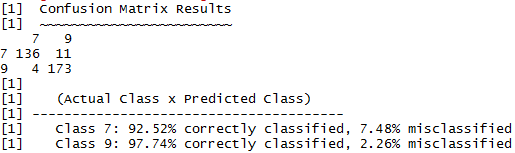
\includegraphics[width=.8\linewidth]{7_9_confusion}
  \caption{A custom confusion-matrix-output from R indicating the classification performance of the Fisher Discriminant on 7s and 9s.}
  \label{fig:7_9_confusion}
\end{figure}

%
\newpage
\subsection{Code}
The following R code was used to perform the LDA and classification:
\begin{verbatim}
##############
# STAT775: Machine Learning
#
# Exercise 02
#
# Using the zip code digit data from the ESL website, use the Fisher
# Discriminant to perform binary classification between 2s and 3s, 4s and 5s,
# and 7s and 9s.
###############

#
# Initial Setup
#
setwd('C:/Users/Terence/Documents/GitHub/STAT775/HW04')
FILE.PRE <- 'zip.data/zip'

rdm <- function(relative.file.name, class, extension) {
  return(data.matrix(read.table(
    paste(relative.file.name, class, extension, sep = '.'),
    sep = ',',
    header = F
  )))
}


read.data.summary <- function(relative.file.name, class, extension) {
  data <- rdm(relative.file.name, class, extension)

  mean = data.matrix(colMeans(data))
  covariance = cov(data)

  summary <- list(freq = nrow(data), mu = mean, sigma = covariance, label = class)
  return(summary)
}


compute.data.summary <- function(data, label) {
  mean = data.matrix(colMeans(data))
  covariance = cov(data)

  summary <- list(
    freq = nrow(data),
    mu = mean,
    sigma = covariance,
    label = label
  )
  return(summary)
}


gaussian.pdf <- function(x, mu, sigma) {
  p <- nrow(sigma)
  sig.ma <- sigma

  det.sigma <- det(sig.ma)
  if (det.sigma < 0.0001) {
    sig.ma <- sig.ma + diag(0.0001, nrow(sig.ma), nrow(sig.ma))
    det.sigma <- det(sig.ma)
  }

  scale.factor <- 1.0 / sqrt((2 * pi)^p * det.sigma)
  exponent <- t(x - mu) * solve(sigma) * (x - mu)

  return(scale.factor * exp(exponent))
}


unscaled.naive.bayes.pdf <- function(x, class.info, n.obs) {
  return(
    gaussian.pdf(x = x, mu = class.info$mu, sigma = class.info$sigma) *
    (class.info$freq / n.obs)
  )
}

#
# Classifier Implementation
#
library(ppls)  # for vector normalization

create.fisher.discriminant.model <-
function(c0, c1, use.naive.db = T, c0.data = NULL, c1.data = NULL) {
  sigma.sum <- (c0$sigma + c1$sigma)
  if (abs(det(sigma.sum)) < 0.001) {
    sigma.sum <- sigma.sum + diag(0.1, nrow = nrow(sigma.sum))
  }
  fisher.discriminant <- normalize.vector(solve(sigma.sum) %*% (c0$mu - c1$mu))

  discriminant.c0 <- NULL
  discriminant.c1 <- NULL
  decision.boundary <- NULL
  if(use.naive.db) {
    discriminant.c0 <- c0
    discriminant.c1 <- c1
    decision.boundary <- t(fisher.discriminant) %*% (0.5 * (c0$mu + c1$mu))
  } else {
    projected.data <- t(t(fisher.discriminant) %*% t(c0.data))
    discriminant.c0 <- list(
      mu = mean(projected.data),
      sigma = var(projected.data),
      freq = c0$freq,
      label = c0$label
    )
    projected.data <- t(t(fisher.discriminant) %*% t(c1.data))
    discriminant.c1 <- list(
      mu = mean(projected.data),
      sigma = var(projected.data),
      freq = c1$freq,
      label = c1$label
    )
    sigma.ratio <- (discriminant.c1$sigma / discriminant.c0$sigma)
    k <- sqrt(log(sigma.ratio)) * sigma.ratio
    decision.boundary <- (k * (discriminant.c0$mu - discriminant.c1$mu)) / (k - 1)
  }

  model <- list(
    fd = fisher.discriminant,
    db = decision.boundary,
    c0 = discriminant.c0,
    c1 = discriminant.c1
  )
  return(model)
}

fisher.predict <- function(model, x, use.naive.db = T) {
  projection <- t(model$fd) %*% data.matrix(x)

  if (use.naive.db) {
    if (projection > model$db) {
      return(model$c0$label)
    } else {
      return(model$c1$label)
    }
  } else {
    if (unscaled.naive.bayes.pdf(c0) - unscaled.naive.bayes.pdf(c1) > 0) {
      return(model$c0$label)
    } else {
      return(model$c1$label)
    }
  }
}

#
# Classifier Testing
#
fisher.discriminant.test <-
function(c0.summary, c1.summary, test.data, test.labels) {
  model <- create.fisher.discriminant.model(c0 = class.0, c1 = class.1)

  classification.results <- matrix(
    data = 0,
    nrow = 2,
    ncol = 2,
    dimnames = list(
      c(c0.summary$label, c1.summary$label),
      c(c0.summary$label, c1.summary$label)
    )
  )

  for (i in 1:length(test.labels)) {
    classified.as <- fisher.predict(model, test.data[i, ])
    previous <- classification.results[test.labels[[i]], classified.as]
    classification.results[test.labels[[i]], classified.as] <- previous + 1
  }

  return(classification.results)
}

print.confusion.result <- function(confusion.matrix) {
  print(' Confusion Matrix Results', quote = F)
  print(' ~~~~~~~~~~~~~~~~~~~~~~~~', quote = F)
  print(confusion.matrix)
  print('', quote = F)
  print('   (Actual Class x Predicted Class)', quote = F)
  print('---------------------------------------', quote = F)

  class.totals <- rowSums(confusion.matrix)
  for (i in 1:length(class.totals)) {
    correct.rate <- confusion.matrix[i, i] / class.totals[[i]]
    class.result.str <- sprintf(
      '   Class %s: %.2f%% correctly classified, %.2f%% misclassified',
      row.names(confusion.matrix)[[i]],
      correct.rate * 100,
      (1 - correct.rate) * 100
    )
    print(class.result.str, quote = F)
  }
}

plot.fisher.test.result <- function(confusion.matrix) {
  names <- row.names(confusion.matrix)
  totals <- rowSums(confusion.matrix)
  rates <- list()
  rates[[1]] <- confusion.matrix[1, 1] / totals[[1]]
  rates[[2]] <- confusion.matrix[1, 2] / totals[[1]]
  rates[[3]] <- confusion.matrix[2, 2] / totals[[2]]
  rates[[4]] <- confusion.matrix[2, 1] / totals[[2]]

  plot.data <- data.frame(
    'Actual' = c(names[[1]], names[[1]], names[[2]], names[[2]]),
    'Predicted' = c(names[[1]], names[[2]], names[[2]], names[[1]]),
    'Rate' = c(rates[[1]], rates[[2]], rates[[3]], rates[[4]])
  )

  require(ggplot2)
  plot.title <- paste(
    'Fisher Discriminant Performance on Digits ',
    paste(names[[1]], names[[2]], sep = ', '),
    sep = ''
  )
  result.plot <- ggplot(
    data = plot.data,
    aes(x=Actual, y=Rate, fill=Predicted)
    ) +
    geom_bar(
      colour = 'black',
      stat = 'identity',
      position = position_dodge(),
      size = .3
    ) +
    scale_fill_hue(name='Classified As') +
    scale_y_continuous(limits = c(0, 1), breaks = seq(0, 1, 0.025)) +
    xlab('Actual Class') +
    ylab('Classification Rate') +
    ggtitle(plot.title) +
    theme_bw()

  ggsave(
    plot = result.plot,
    filename = paste(gsub(' ', '_', plot.title), 'png', sep = '.')
  )
}

#
# The Whole Shebang
#
zip.train <- (read.table(
  file = 'zip.data/zip.train',
  header = F
))

zip.test <- (read.table(
  file = 'zip.data/zip.test',
  header = F
))

trials <- list(
  list(2, 3),
  list(4, 5),
  list(7, 9)
)

for (trial in trials) {
  class.0.data <- data.matrix(subset(zip.train, V1 == trial[[1]]))[, -1]
  class.1.data <- data.matrix(subset(zip.train, V1 == trial[[2]]))[, -1]

  class.0 <- compute.data.summary(data = class.0.data, label = as.character(trial[[1]]))
  class.1 <- compute.data.summary(data = class.1.data, label = as.character(trial[[2]]))

#   model <- create.fisher.discriminant.model(
#     c0 = class.0,
#     c1 = class.1
#   )
  model <- create.fisher.discriminant.model(
    c0 = class.0,
    c1 = class.1,
    use.naive.db = F,
    c0.data = class.0.data,
    c1.data = class.1.data
  )

  test.set <- data.matrix(subset(zip.test, V1 == trial[[1]] | V1 == trial[[2]]))
  test.data <- test.set[, -1]
  test.labels <- lapply(as.list(test.set[, 1]), as.character)

  confusion.matrix <- fisher.discriminant.test(
    c0.summary = class.0,
    c1.summary = class.1,
    test.data = test.data,
    test.labels = test.labels
  )

  print.confusion.result(confusion.matrix)
  plot.fisher.test.result(confusion.matrix)
}
\end{verbatim}

\end{document}
